%% 背景： LLM很强，但并未充分利用到GPU的计算能力
While large language models have achieved expert-level performance on reasoning, coding, and long-context tasks \citep{singh2025openai}, their standard 
autoregressive decoding remains inherently sequential. This process is often memory-bound, leaving the massive parallelism of modern GPUs underutilized and leading to 
high inference latency.
\begin{figure}[t]
    \centering
    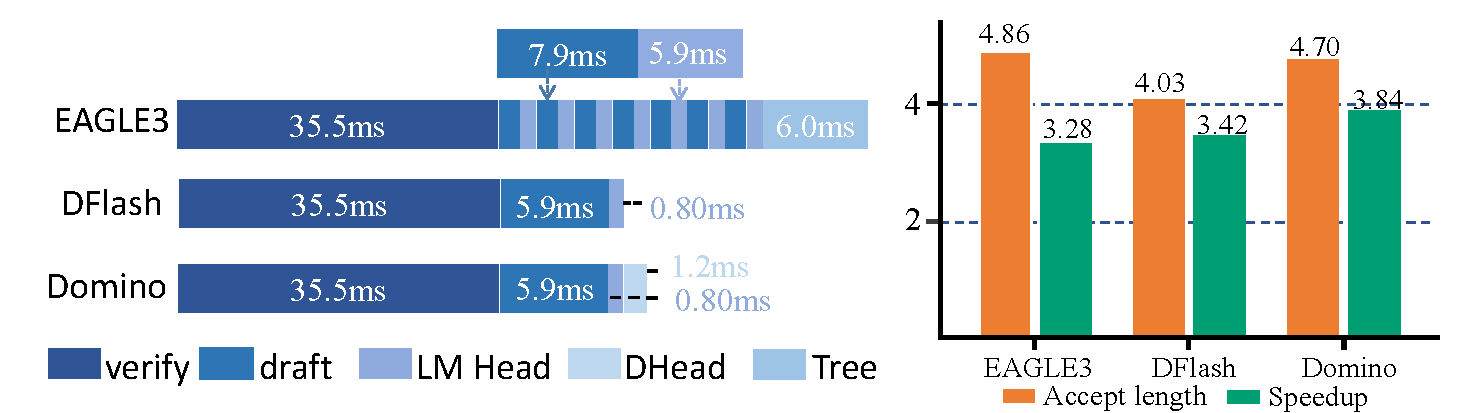
\includegraphics[width=\columnwidth]{latex/figure/domino_overhead.pdf}
    \caption{
    Latency breakdown and performance comparison on Qwen3-8B under a 16-token speculative decoding budget.
    Left: per-step latency breakdown measured on an A100 GPU with context length 1024, where \emph{Verify} denotes the target-model verification latency and \emph{Draft} denotes the draft-model forward latency.
    \emph{LM Head}, \emph{DHead}, and \emph{Tree} denote the output projection, Domino head, and tree construction/sampling overheads, respectively.
    Right: acceptance length and end-to-end speedup evaluated on GSM8K.
    All three draft models are trained on the same dataset.
    }


    \label{fig:draft_overhead}
    \vspace{-2mm}
\end{figure}
\begin{figure*}[t]
  \centering
  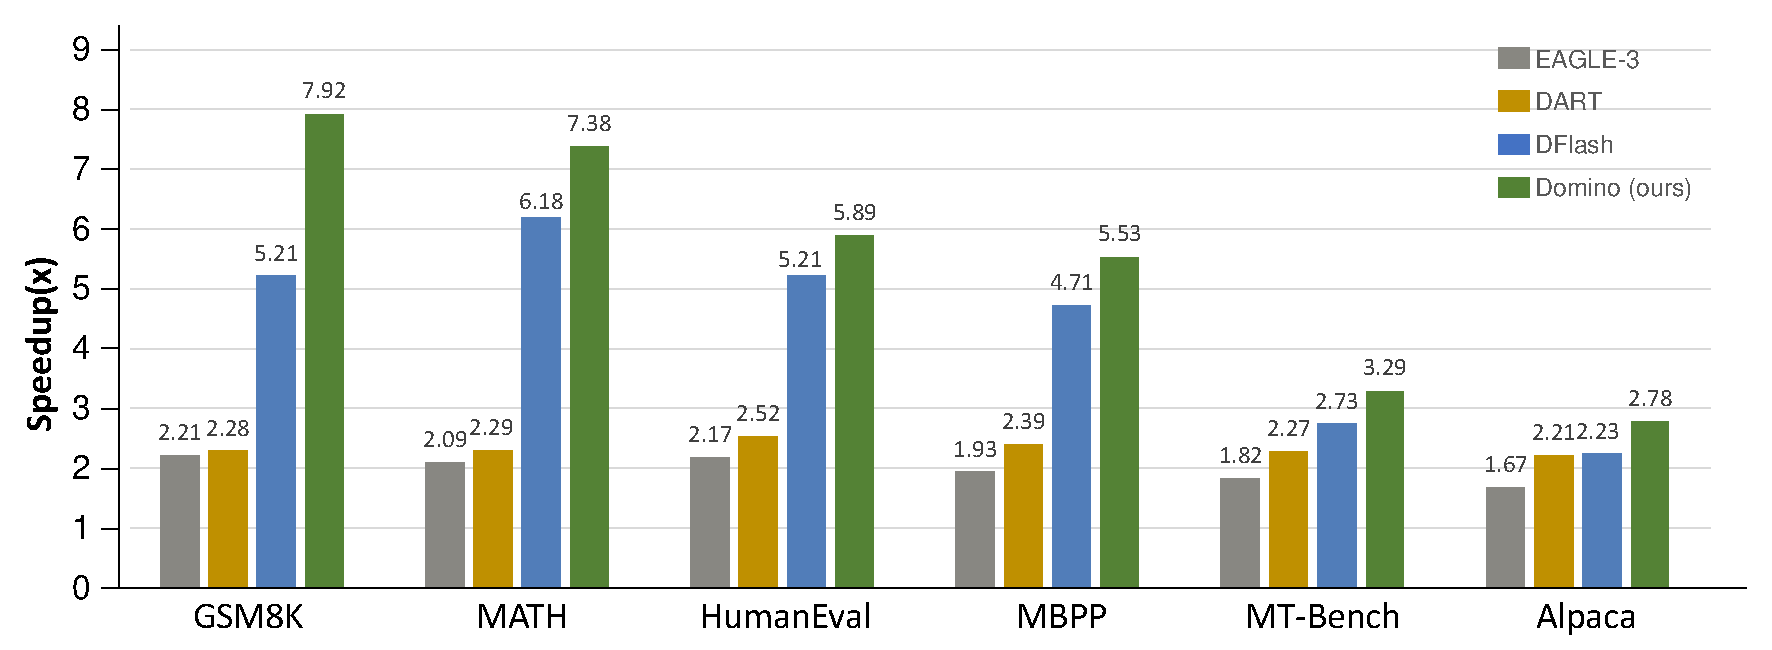
\includegraphics[width=1.0\linewidth]{latex/figure/speedup.pdf}
  \caption{Speedup comparison of Domino, DFlash, and EAGLE-3 relative to autoregressive decoding on Qwen3-8B using the Transformers backend.}
  \label{fig:domino_intro}
\end{figure*}
%% 背景：为了解决这个问题，speculative decoding出现
To alleviate this bottleneck, speculative decoding has emerged as a widely adopted strategy for accelerating LLM inference \citep{leviathan2023fast}. It leverages a lightweight draft model to propose multiple future tokens, which are then verified in parallel by the target model within a single forward pass. By reducing the number of expensive invocations of the target model, this draft-then-verify mechanism preserves the target model's output distribution while improving throughput. Subsequent work has explored various drafting strategies, including head-based multi-token prediction \citep{cai2024medusa} and autoregressive draft models \citep{li2024eagle, li2024eagle2, li2025eagle3}. Across these methods, the resulting speedup is jointly determined by two factors: \emph{draft quality and drafting cost}. Higher-quality drafts yield longer acceptance lengths, but the drafting process itself introduces additional overhead that can diminish or even negate these gains.

This quality--cost trade-off is especially evident in autoregressive drafting methods such as the EAGLE series \citep{li2024eagle, li2024eagle2, li2025eagle3}. By generating draft tokens sequentially, autoregressive drafters explicitly model causal dependencies within the draft block, improving alignment with the target model's autoregressive distribution and yielding long acceptance lengths. However, generating \(k\) draft tokens requires \(k\) sequential draft steps, each involving a draft-model forward pass and a full-vocabulary LM-head projection. This cost grows linearly with draft length and can offset the gains from higher acceptance length, limiting the speedup obtained by scaling draft length or draft capacity \citep{zhao2025fr,yan2025scaling}.





% \begin{figure*}[t]
%   \centering
%   \includegraphics[width=1.0\linewidth]{latex/figure/domino_intro.svg}
%   \caption{Speedup comparison between Domino, DFlash, EAGLE-3 against Autoregressive Decoding on Qwen3-8B with the Transformers backend.} 
%   \label{fig:pipe_figure}
% \end{figure*}

Existing methods address this issue from different directions. FR-Spec \citep{zhao2025fr} and SpecVocab \citep{williams2026speculative} reduce the cost of full-vocabulary projection through static or dynamic vocabulary selection, but still retain autoregressive draft execution. In contrast, DFlash \citep{chen2026dflash} fully parallelizes drafting by producing an entire draft block in one forward pass, avoiding repeated per-token draft-model and LM-head calls. However, removing sequential draft dependencies weakens intra-block causal modeling and can reduce the alignment between the draft distribution and the target model distribution.

Figure~\ref{fig:draft_overhead} illustrates this trade-off. 
EAGLE-3 obtains a high acceptance length of \(4.86\), but its sequential draft execution and tree construction limit the speedup to \(3.28\times\). 
DFlash reduces drafting overhead through block-parallel generation and improves speedup to \(3.42\times\), but its acceptance length decreases to \(4.03\). 
These results suggest that causal dependency modeling is useful for draft quality, but the standard autoregressive implementation makes it expensive. 
This raises a natural question: can we retain the draft-quality benefit of causal dependency modeling while preserving the low drafting cost of block-parallel generation?

To answer this question, we propose Domino, a lightweight causal correction framework that decouples causal dependency modeling from expensive autoregressive draft execution. Instead of generating draft tokens sequentially, Domino keeps the main drafting computation parallel: a parallel draft backbone first produces preliminary draft distributions for the entire block. On top of these distributions, Domino applies a lightweight Domino head to inject causal information. The Domino head uses a causal encoder to summarize previously drafted tokens and a low-rank correction head to refine the draft distributions through residual correction, avoiding repeated draft-model execution and another expensive full LM-head computation.

This design allows Domino to recover useful intra-block causal dependency while preserving the efficiency of block-parallel drafting. As shown in Figure~\ref{fig:draft_overhead}, compared with DFlash, Domino adds only 56M parameters (+5.3\%) and incurs only a 2.8\% increase in total draft-then-verify latency. Simultaneously, it improves average acceptance length by 16.6\% and end-to-end speedup by 12.3\%. 

Figure~\ref{fig:domino_intro} provides a preview of the empirical gains. 
On representative math, code, and chat benchmarks, Domino consistently outperforms EAGLE-3, DART, and DFlash, achieving up to \(7.92\times\) speedup on GSM8K and improving over DFlash from \(5.21\times\) to \(7.92\times\). 
These results suggest that lightweight causal correction improves draft quality while preserving the efficiency of block-parallel drafting.
% Overall, our main contributions are summarized as follows.


% Our contributions are summarized as follows.
% \begin{enumerate}
% \item We identify the trade-off between draft quality and drafting cost in speculative decoding: causal modeling improves draft quality, but sequential execution limits speedup.

% \item We propose \textsc{Domino}, which injects lightweight causal correction into parallel drafting, improving draft quality while maintaining low drafting overhead.

% \item Experiments on diverse tasks show that \textsc{Domino} consistently achieves state-of-the-art performance, with up to \(7.92\times\) speedup on GSM8K.
% \end{enumerate}